
\chapter{STABILITY AND RECONSTRUCTIONS OF PT/PD BIMETALLIC NANOCUBES EXPOSED TO CARBON MONOXIDE}

\section{Introduction}

While metal surfaces are used in various industrial processes, because of their
poor surface area to volume ratio, many methods make use of roughened surfaces
or more preferrably nanoparticles dispersed on a cheaper unreactive surface.\cite{} The size distribution of the
nanoparticles can vary but tends to be on the order of tens to hundredes of nanometers
in size.\citep{} Additionally, the morphology of these nanoparticles spans from simple
cubes, to octahedra, pyramids, and numerous other morphologies.\citep{} As seen
in previous work\citep{Tao:2010aa, Michalka:2013aa, Michalka:2015aa, Kim:2016cr}, even fairly stable surfaces can undergo
large scale reconstructions under experimental conditions. This appendix
provides information on the initial setup of bimetallic Pt/Pd nanocubes and the
preliminary results obtained before the project was shelved. 

\section{Methodology}
\subsection{Interaction Parameters}
The interaction potentials provided in Michalka {\em et al.}\citep{Michalka:2015aa} are used here unchanged. 

\subsection{System Details}
Nanocubes with edge lengths of 6, 7, and 8 nm were constructed from an ideal \ce{Pd}
FCC lattice with a lattice constant of 3.89 \AA~  and cut so as to expose the
(100), (010), and (001) facets. For each of these three sizes, the outermost 1,
2, or 3 layers were further replaced with Pt to create nine total systems whose compositions
are depicted in table \ref{tab:systems}. Work by Cao {\it et al.}\citep{Cao:2010gf} on the
self-distillation of bimetallic nanostructures showed that when the outer shell
of nanoparticles was composed of the metal with a higher melting temperature,
it imposed stability on the confined inner metal. For this reason, Pt was
chosen to compose the outer layers while keeping the core of the nanoparticle
Pd. Additionally, the slightly more favorable Pd-CO interaction may provide a
driving force for reconstructions that will be dependent on the thickness of
the Pt since Pd will want to migrate through the Pt to the surface.

\begin{table}
  \caption{PT/PD NANOCUBE SIZES AND COMPOSITION}
  \centering
  \begin{threeparttable}
  \begin{tabular}{ c ccc }
  \hline
  \hline
  \textbf{System} & \textbf{Pd} & \textbf{Pt} &  \textbf{(Pt/total)} \\
  \hline
  6nm-1L & 10976 & 2524  & 0.187 \\
  6nm-2L & 8788  & 4712  & 0.349 \\
  6nm-3L & 6912  & 6588  & 0.488 \\
  7nm-1L & 19652 & 3676  & 0.157 \\
  7nm-2L & 16384 & 6944  & 0.298 \\
  7nm-3L & 13500 & 9828  & 0.421 \\
  8nm-1L & 27436 & 4564  & 0.143 \\
  8nm-2L & 23328 & 8672  & 0.271 \\
  8nm-3L & 19652 & 12348 & 0.386 \\
  \hline
  \hline
  \end{tabular}
  \end{threeparttable}
\label{tab:systems}
\end{table}

Systems were constructed in a non-periodic box and then initially equilibrated
at 5~K to allow the slight strain of replacing Pd atoms with Pt in the outer
layers to dissipate. Warming over approximately 3~ns was performed to bring all systems up to
a simulation temperature of 1000~K at which point an amount of Carbon
Monoxide equivalent to a 0.5 ML coverage was introduced into the system.
After another brief period of equilibration during which a
significant amount of the CO adsorbed to the surface, the systems were then run
in the microcanonical (NVE) ensemble for an additional 3~ns of data production.

Figures \ref{fig:6nm}, \ref{fig:7nm}, and \ref{fig:8nm} highlight the nanocube
systems after the initial strain relaxation and then after the systems have
been warmed. The instability of the smaller systems as highlighted in Figure
\ref{fig:6nm} is what led to the pausing of this project. Additionally, for the
7nm-1L and 8nm-1L systems, only having one layer of \ce{Pt} led to an immediate
reconstruction to a thin layer of (111) \ce{Pt} on top of the underlying (100)
\ce{Pd}.



\begin{landscape}
\begin{figure}[p!]
  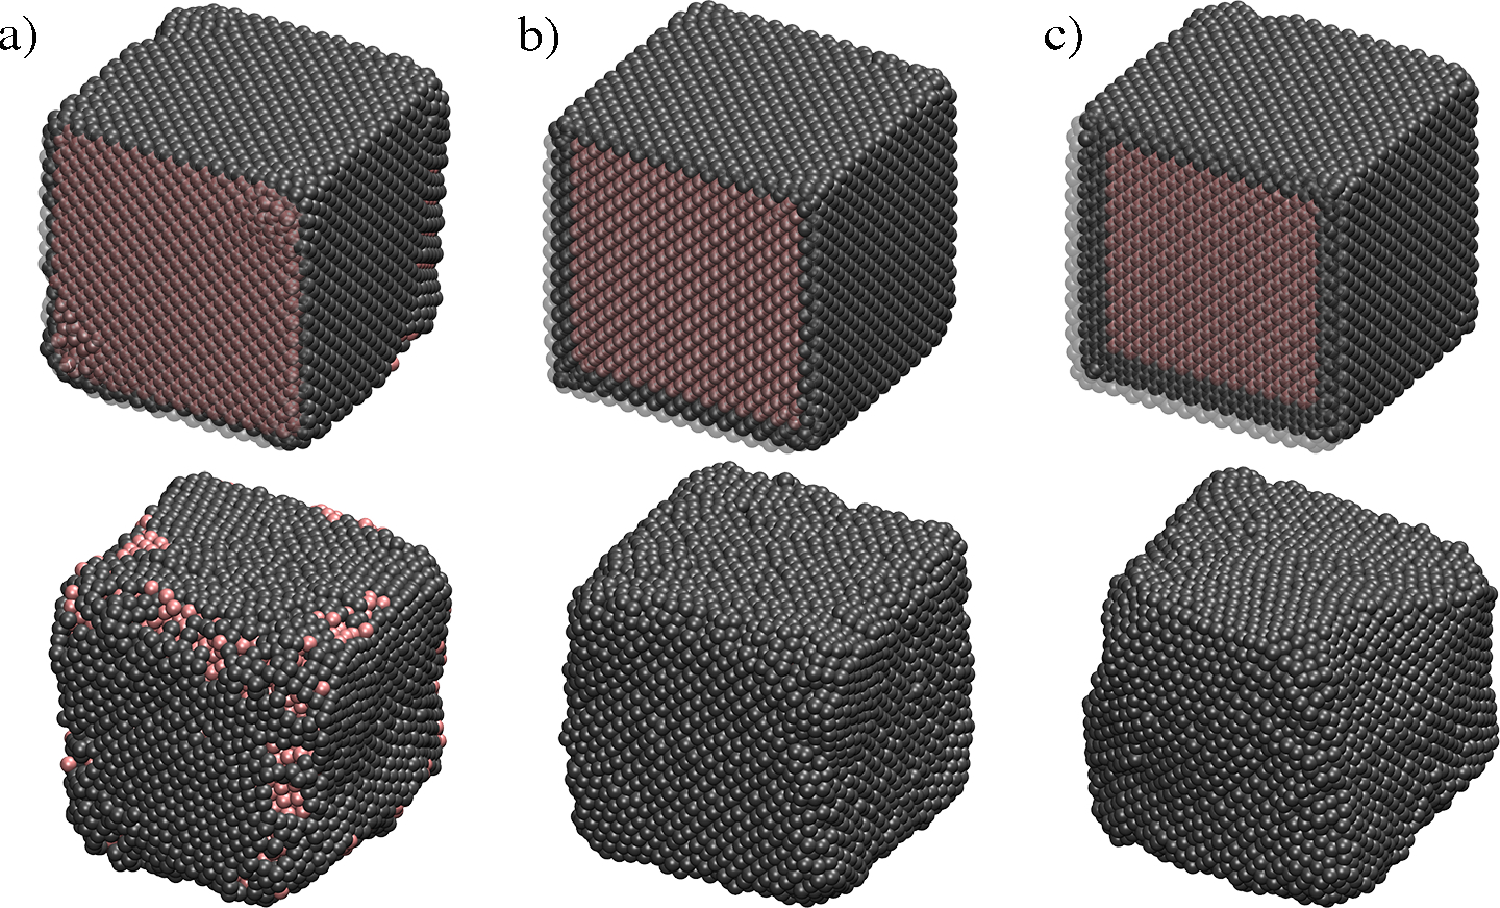
\includegraphics[width=\linewidth]{../figures/appB/6nm.pdf}
  \caption{}
  \label{fig:6nm}
\end{figure}
\end{landscape}


\begin{landscape}
\begin{figure}[p!]
  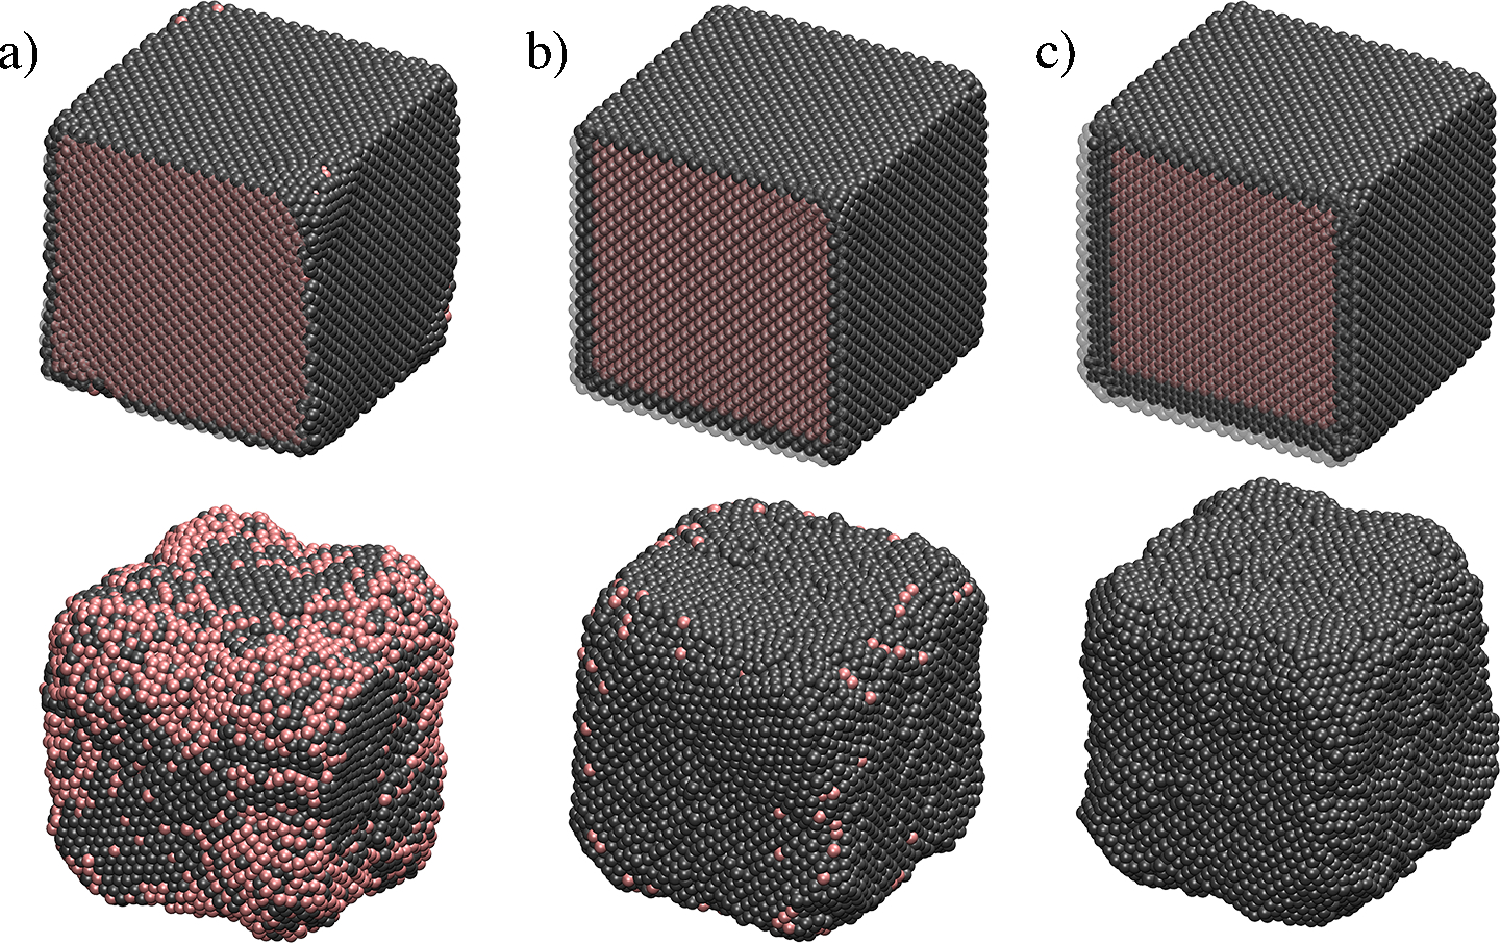
\includegraphics[width=\linewidth]{../figures/appB/7nm.pdf}
  \caption{}
  \label{fig:7nm}
\end{figure}
\end{landscape}


\begin{landscape}
\begin{figure}[p!]
  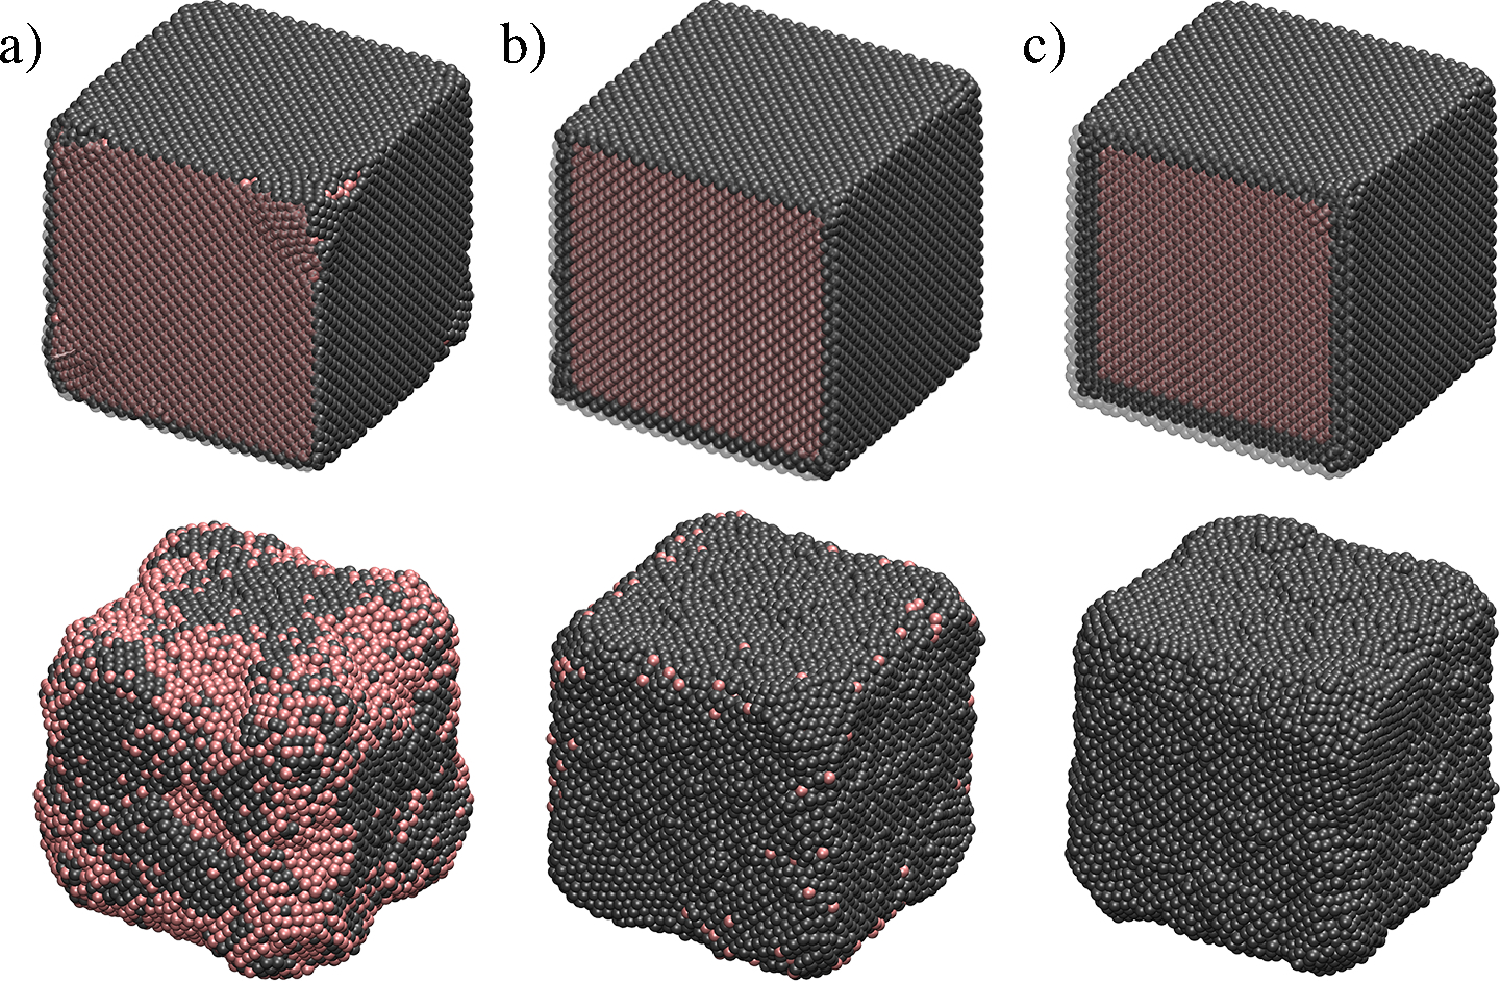
\includegraphics[width=\linewidth]{../figures/appB/8nm.pdf}
  \caption{}
  \label{fig:8nm}
\end{figure}
\end{landscape}



\section{Results \& Discussion}
One of the challenges that ultimately led to this project being shelved is the
size of the systems and the cocommitant increase in simulation time needed to
capture the hypothesized restructuring processes. Nevertheless, preliminary
results were gathered and are discussed below.

\subsection{CO-Induced Reconstruction}
As seen in previous work\citep{Michalka:2013aa}, the presence of CO was again seen to play a
role in the observed restructuring. However, unlike what was observed on the Pt
(557) surface\citep{Michalka:2013aa}, where CO was required for any large-scale reconstruction
to occur, for these systems a significant portion of the reconstruction could
be directly attributed to lower stability of the (100) facets when compared to
(111) facets. As highlighted in Figure \ref{fig:reconstructed}, this system
underwent this extreme amount of reconstruction despite no CO being present. 

\section{Summary}
The observed restructuring while informative, was primarily determined to be an
artifact of the small systems sizes that were chosen for this investigation.
Future simulations examining larger systems (>10 nm) may solve the buckling
observed in a number of these systems. Additionally, an exploration into
octahedral-type nanoparticles with their preponderence to exposed {111} facets
may also help solve the stability issues and provide another direction to explore.
